\clearpage
\section{Books, Processional Items, and Incense}
\PCDPlateHeader{Plate V --- Liturgical Books and Stands}{Relative proportions shown}
\ifdefined\TriptychPrintEdition
\begin{center}
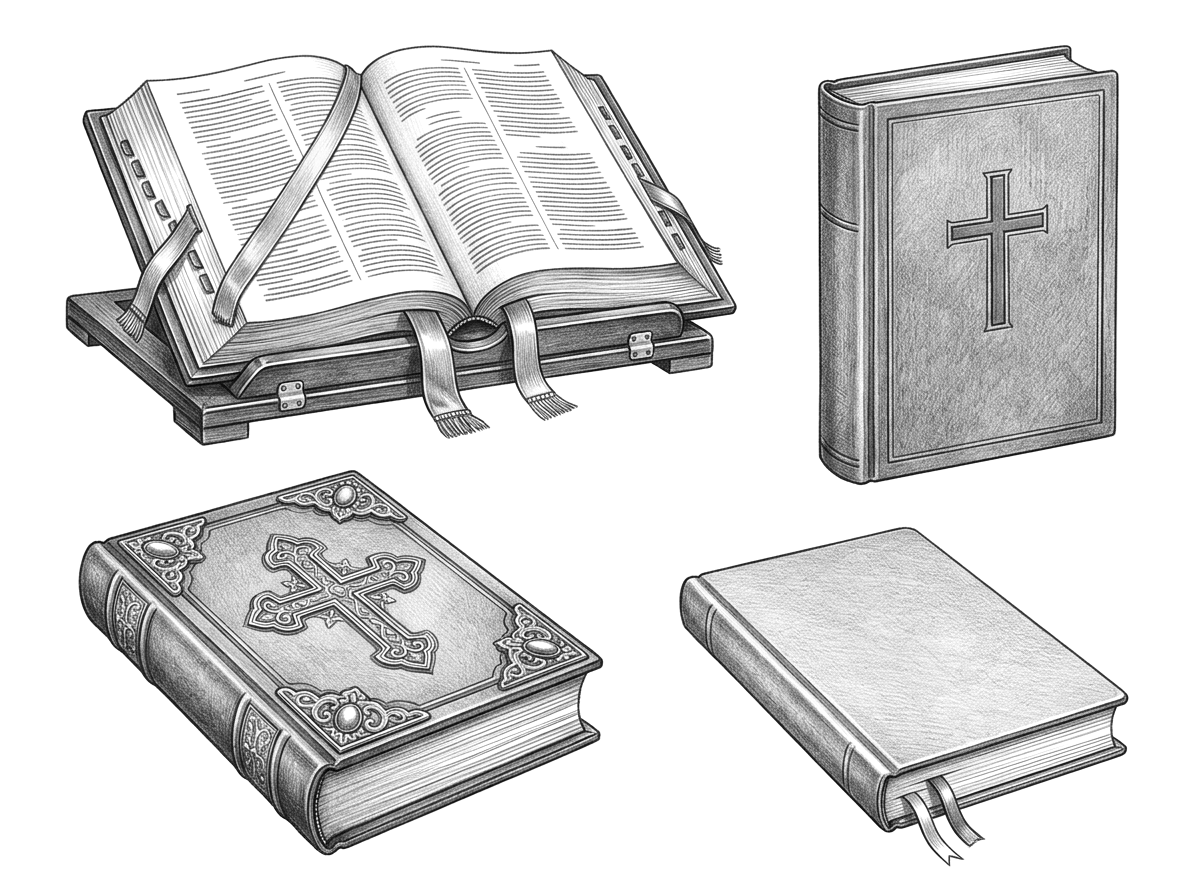
\includegraphics[width=0.92\linewidth,height=3.55in,keepaspectratio]{liturgy/roman-rite/postconciliar/2008-latin-2011-us-english/reference/roman-sanctuary-dictionary/shared/artwork/graphite/pc-art-05-liturgical-books.png}
\end{center}
\PCDPositionKey{Top left: thick Roman Missal open with side tabs and ribbon markers on a low angled Missal Stand; top right: tall closed Lectionary for Mass; bottom left: ornate bound Book of the Gospels (Evangeliary) with metal corner bosses and embossed cross; bottom right: slimmer Book of the Chair (Excerpts from the Roman Missal).}
\else
\textbf{Visual Plate Summary (Plate V --- Liturgical Books and Stands, Relative proportions shown):} Four-book monochrome graphite comparison showing relative scale and binding dignity: top left, a thick altar Roman Missal open flat with ribbon markers and edge tabs on a low angled wooden stand; top right, a tall closed hardcover Lectionary marked with a plain cover cross; bottom left, a heavily ornamented Book of the Gospels with sculpted metal corner bosses and central embossed cross; bottom right, a slimmer handheld Book of the Chair with two ribbon markers.

\textbf{Reading order and object placement:} Top left: thick Roman Missal open with side tabs and ribbon markers on a low angled Missal Stand; top right: tall closed Lectionary for Mass; bottom left: ornate bound Book of the Gospels (Evangeliary) with metal corner bosses and embossed cross; bottom right: slimmer Book of the Chair (Excerpts from the Roman Missal).
\fi

\label{pc-obj-roman-missal}
\PCDEntryHead{Roman Missal}{Missale Romanum}{required}{N20}
\PCDField{Also called}{Altar Missal; Sacramentary (1974--2011 U.S. usage); \textit{Missale}}
Whenever the priest prays the opening Collect at his chair or offers the Eucharistic Prayer at the altar, he reads from the Roman Missal---the Church's authoritative book of Mass prayers. While the Lectionary on the ambo holds the Scripture readings, the Missal gathers the prayers offered by the priest in the name of the entire Church across every season and feast, crafted with lasting dignity and beauty to honor the sacred liturgy (GIRM 349).

\PCDField{On the plate}{Top left, open with edge tabs and ribbons on a low stand (Plate V)}
\PCDField{Symbolism}{The General Instruction of the Roman Missal teaches that liturgical books serve as signs and symbols of heavenly realities, requiring that the Roman Missal be crafted with genuine worth, dignity, and beauty to honor the Eucharistic prayer of the Church. (GIRM 349)}
\PCDField{Relation to the 1962 Missal}{\PCDTag{materially changed} The 1962 Missale Romanum was a plenary altar book holding all presidential orations, chants, Epistles, and Gospels, remaining on the altar throughout Mass and carried between the Epistle and Gospel corners (RG 527; RS VI.5, XI.1). In the postconciliar Roman Rite, the Scripture readings are separated into the Lectionary and Book of the Gospels, while the Missal serves at the presidential chair and rests on the altar only from the Preparation of the Gifts through purification (GIRM 118a, 139, 306).}
\PCDEntryRule

\label{pc-obj-lectionary}
\PCDEntryHead{Lectionary for Mass}{Lectionarium}{required}{N21}
\PCDField{Also called}{Lectionary; \textit{Ordo lectionum Missae}}
Resting open on the ambo before Mass begins, the Lectionary unfolds a wide treasury of Old Testament, Psalm, Apostolic, and Gospel passages arranged over a three-year Sunday cycle and two-year weekday cycle. Together with the altar, the ambo and Lectionary present the table of God's Word from which Christ nourishes the Church before inviting the faithful to the table of his Body (GIRM 28, 349).

\PCDField{On the plate}{Top right, tall closed volume with cover cross (Plate V)}
\PCDField{Symbolism}{The General Instruction of the Roman Missal honors the Lectionary alongside the Book of the Gospels as a sign and symbol of heavenly realities serving the proclamation of God's Word, feeding the faithful at the table of God's Word before the table of Christ's Body. In the words of the psalmist, ``Thy word is a lamp to my feet, and a light to my paths'' (Ps 118:105 [119:105]). (GIRM 28, 349; Ordo lectionum Missae (1981) Praenotanda 35; Ps 118:105 [119:105])}
\PCDField{Relation to the 1962 Missal}{\PCDTag{materially changed} In the 1962 Roman Missal, the one-year cycle of Epistles and Gospels was printed inside the Missal itself, with an optional separate Epistle book (liber Epistolarum) for the subdeacon at Solemn Mass (RS VI.4). The postconciliar reform established a dedicated multi-volume Lectionary spanning a three-year Sunday cycle (A, B, C) and two-year weekday cycle (I, II), placed open on the ambo for every Mass with a congregation (GIRM 118b; OLM 1981).}
\PCDEntryRule

\label{pc-obj-book-of-the-gospels}
\PCDEntryHead{Book of the Gospels}{Evangeliarium}{provided}{N22}
\PCDField{Also called}{Evangeliary; Gospel Book; \textit{Liber Evangeliorum}}
At Sunday and festive Masses, the deacon---or a reader when no deacon is present---carries this richly decorated volume slightly elevated in the entrance procession and lays it directly upon the altar, the only book placed on the altar table during the first half of Mass. Before the Gospel reading, ministers escort it from the altar to the ambo with lighted candles and incense, honoring Christ himself who speaks directly to his people in the proclamation of the Gospel (GIRM 62, 134, 349).

\PCDField{On the plate}{Bottom left, ornate metal-bossed cover (Plate V)}
\PCDField{Symbolism}{First among all liturgical books as a sign and symbol of heavenly realities, the Book of the Gospels receives elevation in procession, placement upon the altar, escort with lights and incense, and a reverent kiss because Christ himself speaks directly to his Church in the Gospel. St. Thomas Aquinas similarly distinguishes the earlier readings as preparatory instruction from the Gospel, by which Christ's own teaching instructs the faithful perfectly. (GIRM 62, 134, 175, 349; St. Thomas Aquinas, Summa Theologiae III, q. 83, a. 4, corpus)}
\PCDField{Relation to the 1962 Missal}{\PCDTag{changed use} In the 1962 Roman Missal, a separate Gospel book (liber Evangeliorum) belonged to Solemn Mass, where it was placed on the altar only before the Gospel, carried by the deacon in the Gospel procession, held by the subdeacon between lighted candles, incensed, and brought to the celebrant to kiss (RS VI.5). Postconciliar rubrics integrate the Book of the Gospels into ordinary Sunday and festive celebrations, carrying it slightly elevated in the entrance procession and resting it on the altar from the start of Mass until the Gospel procession (GIRM 120d, 122, 133--134, 306).}
\PCDEntryRule

\label{pc-obj-book-of-the-chair}
\PCDEntryHead{Book of the Chair}{Excerpts from the Roman Missal (no Latin typical edition)}{territorial adaptation}{N23}
\PCDField{Also called}{Excerpts from the Roman Missal; Presidential Prayer Book}
During the opening and closing prayers of Mass, you will often see an altar server step before the priest at the presidential chair holding a noticeably slimmer book than the thick volume later used at the altar. Officially titled Excerpts from the Roman Missal and published in 2018 for United States dioceses, this practical companion gathers the prayers spoken at the chair while reserving the complete Roman Missal for the altar.

\PCDField{On the plate}{Bottom right, slimmer handheld ceremonial volume (Plate V)}
\PCDField{Relation to the 1962 Missal}{\PCDTag{no established counterpart} Because the priest in the 1962 Roman Missal prayed the Collect and Postcommunion at the altar rather than at a presidential chair (RG 527), there was no presbyteral Book of the Chair (only a minister holding the Missal for a bishop under Caeremoniale Episcoporum I.20). The Holy-See-confirmed USCCB volume Excerpts from the Roman Missal (2018) is a distinct postconciliar practical companion fulfilling GIRM 118a.}
\PCDEntryRule

\label{pc-obj-missal-stand}
\PCDEntryHead{Missal Stand}{Pulpitum}{customary}{N24}
\PCDField{Also called}{Altar bookstand; Missal cushion; \textit{Legile}; \textit{Cussinus}}
This low angled wooden rest---or, in some churches, a firm tailored cushion---supports the heavy Roman Missal at a legible slope for the priest during the Liturgy of the Eucharist. It remains off the altar during the first half of Mass so the mensa stays uncluttered, and its low height preserves an unobstructed view of the Eucharistic action (GIRM 306--307).

\PCDField{On the plate}{Top left, low angled stand beneath the open Missal (Plate V)}
\PCDField{Relation to the 1962 Missal}{\PCDTag{continued} The Missal stand or cushion continues in practical form from the 1962 Roman Missal, which expressly required a cushion or bookstand beneath the Missal on the altar from the start of Mass and directed the server to move it from the Epistle side to the Gospel side and back (RG 527; RS VI.5, XI.1). In the postconciliar Roman Rite, it is neither mandated by name nor kept on the altar before the Preparation of the Gifts, but set once on the mensa for the Liturgy of the Eucharist and removed afterward (GIRM 139, 306).}
\PCDEntryRule

\clearpage
\PCDPlateHeader{Plate VI --- Processional and Service Equipment}{Not to common scale}
\ifdefined\TriptychPrintEdition
\begin{center}
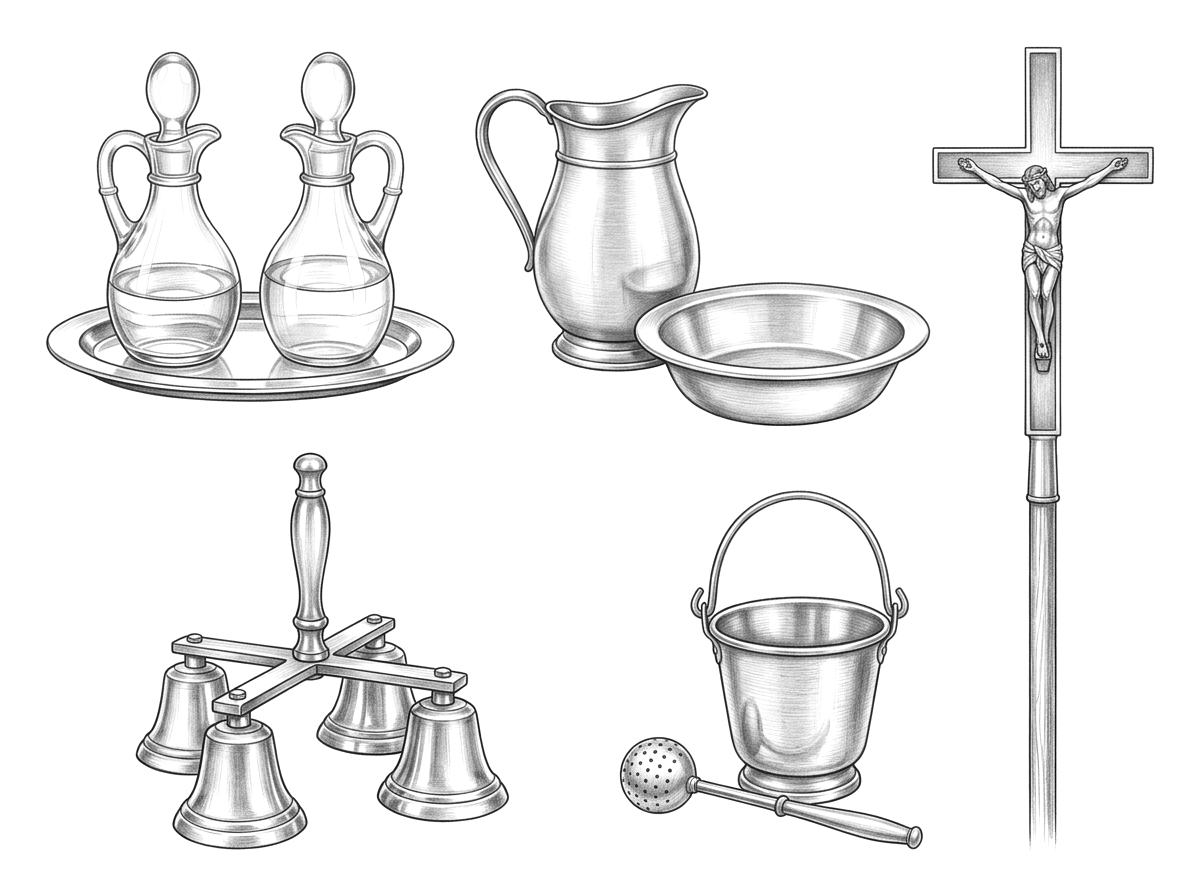
\includegraphics[width=0.92\linewidth,height=3.55in,keepaspectratio]{liturgy/roman-rite/postconciliar/2008-latin-2011-us-english/reference/roman-sanctuary-dictionary/shared/artwork/graphite/pc-art-06-service-cruets-bells.png}
\end{center}
\PCDPositionKey{Top left: paired glass wine and water Cruets with stoppers on a tray; top center: Lavabo pitcher and shallow finger basin; top right: Processional Cross bearing the sculpted corpus of Christ on a staff; bottom left: four-cup mounted brass Sanctuary Bell; bottom right: holy-water Aspersorium bucket and perforated metal Aspergillum.}
\else
\textbf{Visual Plate Summary (Plate VI --- Processional and Service Equipment, Not to common scale):} Five-object monochrome graphite service equipment study: top left, two stoppered transparent glass cruets for wine and water resting on an oval metal tray; top center, a metal lavabo pitcher beside a shallow round finger basin; top right, a tall processional cross on a wooden staff bearing the sculpted figure of Christ crucified; bottom left, a traditional four-bell mounted brass sanctuary hand bell; bottom right, a metal holy-water aspersorium bucket with bail handle and perforated spherical-head aspergillum resting beside it.

\textbf{Reading order and object placement:} Top left: paired glass wine and water Cruets with stoppers on a tray; top center: Lavabo pitcher and shallow finger basin; top right: Processional Cross bearing the sculpted corpus of Christ on a staff; bottom left: four-cup mounted brass Sanctuary Bell; bottom right: holy-water Aspersorium bucket and perforated metal Aspergillum.
\fi

\label{pc-obj-processional-cross}
\PCDEntryHead{Processional Cross}{Crux processionalis}{required}{N25}
\PCDField{Also called}{Altar Cross; Crucifix; \textit{Crux cum figura Christi crucifixi}}
At the beginning of Mass, the processional cross leads the entrance of the ministers into the sanctuary, directing the eyes of the assembly to Christ crucified. In the postconciliar Roman Rite, this carried crucifix frequently stands beside the altar throughout Mass as the single altar cross, keeping the saving Passion of the Lord visibly present at the heart of Eucharistic worship (GIRM 122, 308).

\PCDField{On the plate}{Top right, bearing sculpted corpus on wooden staff (Plate VI); altar cross at center (Plate I)}
\PCDField{Symbolism}{The cross adorned with the figure of Christ crucified remains visibly before the assembly during Mass and outside liturgical celebrations so as to recall the saving Passion of the Lord (GIRM 308). St. Paul proclaims, ``But we preach Christ crucified'' (1 Cor 1:23) and ``But God forbid that I should glory, save in the cross of our Lord Jesus Christ'' (Gal 6:14), through whom God reconciles all things, ``making peace through the blood of his cross'' (Col 1:20). St. Thomas Aquinas affirms that the consecration of the Eucharist, the acceptance of the sacrifice, and all its fruits flow from the virtue of the Cross of Christ. (GIRM 308; 1 Cor 1:23; Gal 6:14; Col 1:20; St. Thomas Aquinas, Summa Theologiae III, q. 83, a. 5, ad 3)}
\PCDField{Relation to the 1962 Missal}{\PCDTag{changed use} Whereas the 1962 Roman Missal required a separate crucifix standing in the center of the altar (RG 527) and did not ordinarily prescribe a carried cross at a priest's High Mass entrance, the 2002/2008 GIRM assigns the processional cross with the figure of Christ crucified a regular place in the entrance procession (GIRM 120b) and permits it to stand near the altar as the sole altar cross (GIRM 122, 308). The 2002 third typical edition also restored the explicit requirement of the sculpted corpus that had been omitted in the 1970 and 1975 editions.}
\PCDEntryRule

\label{pc-obj-altar-candles}
\PCDEntryHead{Altar Candles}{Candelabra cum cereis}{required}{N26}
\PCDField{Also called}{Altar Candlesticks; Processional Candles; \textit{Cerei}; \textit{Candelabra}}
Lighted candles burn on or near the altar at every Mass, scaling from two on ordinary weekdays to four or six on Sundays and solemnities, and seven when the Diocesan Bishop celebrates (GIRM 117). Carried alongside the cross at the entrance and around the ambo for the Gospel, their living flames honor the presence of Christ in His Word and His Eucharistic sacrifice.

\PCDField{On the plate}{See Plate I, flanking the freestanding altar}
\PCDField{Symbolism}{Candles are lighted at every liturgical celebration to express reverence and festive honor before God (GIRM 117, 307). Their living flame recalls Christ, who declares in the Gospel, ``I am the light of the world. He that followeth me walketh not in darkness, but shall have the light of life'' (John 8:12). (GIRM 117, 307; John 8:12)}
\PCDField{Relation to the 1962 Missal}{\PCDTag{materially changed} Both the 1962 Roman Missal (RG 527) and the 2002/2008 GIRM (117, 307) scale candle counts from two up to six, or seven for the Diocesan Bishop. In 1962, altar candlesticks stood directly on the altar or its gradine flanking the central crucifix, supplemented by separate Sanctus and elevation torches; postconciliar GIRM 117, 122, and 307 permit candlesticks to stand either on or around the altar---including processional candlesticks placed near it---so that the faithful maintain an unobstructed view of the altar table.}
\PCDEntryRule

\label{pc-obj-sanctuary-bells}
\PCDEntryHead{Sanctuary Bells}{Campanula}{optional}{N27}
\PCDField{Also called}{Altar Bell; Sanctus Bell; \textit{Parva campanula}}
During the hushed stillness of the Eucharistic Prayer, the clear ring of small brass sanctuary bells draws the attention of the entire assembly toward the altar at the moment of consecration. Under GIRM 150, ringing the bell shortly before the consecration and at the elevations of the Host and Chalice is an optional practice governed by local custom.

\PCDField{On the plate}{Bottom left, four-cup mounted brass altar bell (Plate VI)}
\PCDField{Relation to the 1962 Missal}{\PCDTag{optional} Whereas the 1962 Roman Missal required a small bell on the Epistle-side table and prescribed ringing at the Sanctus and elevations (RG 528; RS VII.8, VIII.6), the 2002/2008 GIRM makes the bell optional according to local custom---shortly before the consecration and at each showing of the Host and Chalice---omitting the mandatory Sanctus and Communion rings (GIRM 150).}
\PCDEntryRule

\label{pc-obj-aspergillum-aspersorium}
\PCDEntryHead{Aspergillum and Aspersorium}{Aspergillum et aspersorium}{optional}{N28}
\PCDField{Also called}{Holy-Water Sprinkler and Bucket; Holy-Water Vessel; \textit{Vas aquae benedicendae}; \textit{Vas aquae benedictae}}
On Sundays---especially during the fifty days of Easter Time---the priest may bless water during the Introductory Rites and walk down the aisle sprinkling the congregation with this metal bucket and perforated sprinkler (GIRM 51). This shower of blessed water recalls every baptized Christian's entry into Christ's death and resurrection.

\PCDField{On the plate}{Bottom right, holy-water bucket and perforated sprinkler (Plate VI)}
\PCDField{Symbolism}{The bucket and sprinkler are practical service instruments; the sacred symbolism belongs to the sprinkling rite itself, which recalls the grace and cleansing of Baptism (GIRM 51; Roman Missal, Appendix II). Its classic antiphon echoes the Psalmist: ``Thou shalt sprinkle me with hyssop, and I shall be cleansed: thou shalt wash me, and I shall be made whiter than snow'' (Ps 50:9 [Heb 51:7]). (GIRM 51; Roman Missal, Appendix II; Ps 50:9 [Heb 51:7])}
\PCDField{Relation to the 1962 Missal}{\PCDTag{changed use} Although the portable metal bucket and sprinkler continue unchanged in form, the 1962 Roman Missal placed the Sunday Asperges me or Vidi aquam before the start of Mass, with the water blessed in the sacristy and the celebrant wearing a cope before putting on the chasuble. In the 2002/2008 Roman Missal, the Blessing and Sprinkling of Water takes place inside the Introductory Rites in place of the Penitential Act, celebrated by the priest already vested in his chasuble (GIRM 51, 118c; Appendix II).}
\PCDEntryRule

\clearpage
\PCDPlateHeader{Plate VII --- Incense Equipment}{Not to common scale}
\ifdefined\TriptychPrintEdition
\begin{center}
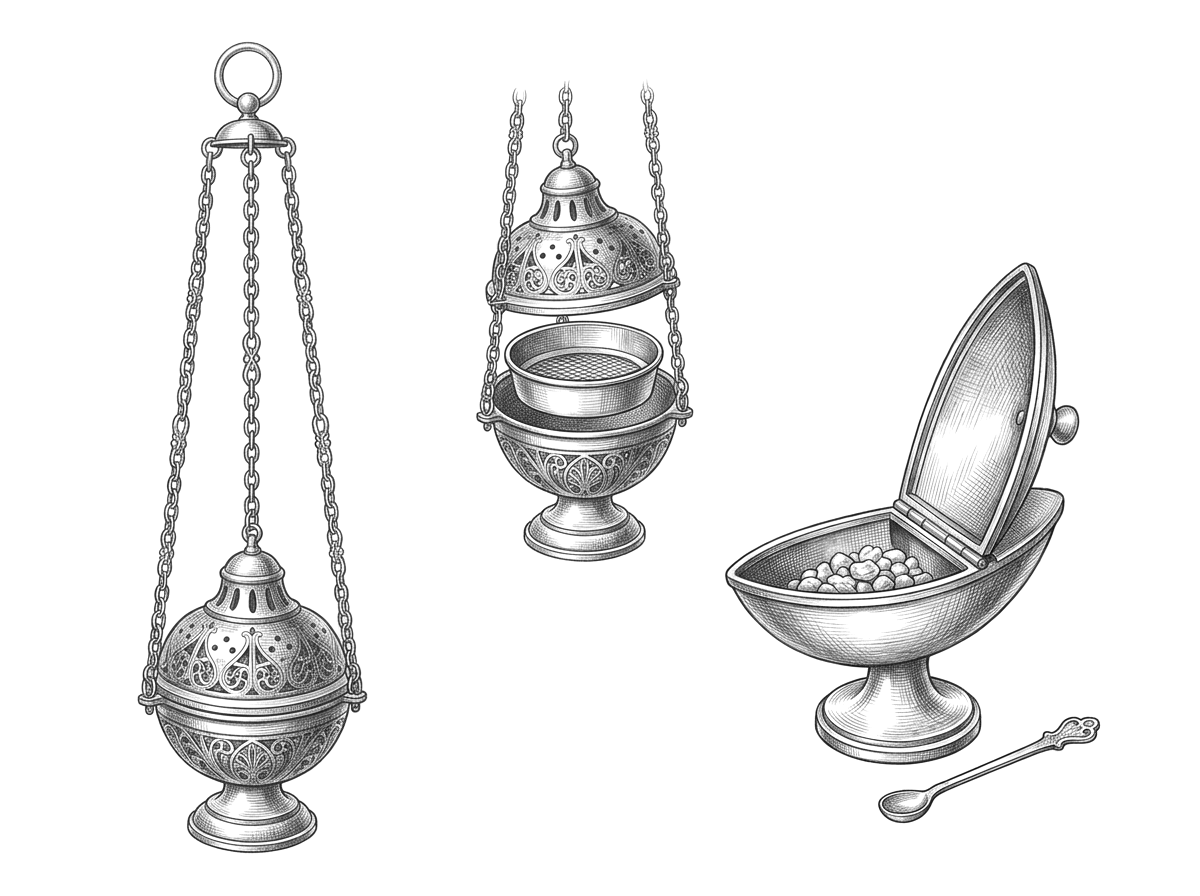
\includegraphics[width=0.92\linewidth,height=3.55in,keepaspectratio]{liturgy/roman-rite/postconciliar/2008-latin-2011-us-english/reference/roman-sanctuary-dictionary/shared/artwork/graphite/pc-art-07-incense-set.png}
\end{center}
\PCDPositionKey{Left: closed metal Thurible suspended on outer rim chains (two visible in profile) and one central lid-lifting chain; center: detail of raised perforated dome revealing removable inner charcoal fire-pan; right: footed Incense Boat (navicula) with hinged half-lid open showing resin grains, accompanied by its metal spoon.}
\else
\textbf{Visual Plate Summary (Plate VII --- Incense Equipment, Not to common scale):} Three-part monochrome graphite incense study: left, a classical footed metal thurible hanging vertically from its top ring on outer rim chains (two visible in profile) and a central lid-lifting chain with perforated domed cover closed; center, a sectional open view with the dome lifted to expose the removable circular charcoal fire-pan; right, a pedestal-footed boat-shaped incense boat with hinged half-lid open showing resin incense grains, paired with a small long-handled metal spoon.

\textbf{Reading order and object placement:} Left: closed metal Thurible suspended on outer rim chains (two visible in profile) and one central lid-lifting chain; center: detail of raised perforated dome revealing removable inner charcoal fire-pan; right: footed Incense Boat (navicula) with hinged half-lid open showing resin grains, accompanied by its metal spoon.
\fi

\label{pc-obj-thurible}
\PCDEntryHead{Thurible}{Turibulum}{optional}{N29}
\PCDField{Also called}{Censer; \textit{Thuribulum}}
When clouds of fragrant smoke curl upward from the swinging metal thurible at the entrance, Gospel, Preparation of the Gifts, and consecration, the liturgy enlists the sense of smell alongside sight and sound to honor Christ. In the postconciliar Roman Rite, incense may be used optionally in any Mass---not solely at Solemn High Mass---at five clearly defined moments (GIRM 276).

\PCDField{On the plate}{Left (closed on chains) and center inset (dome lifted revealing inner charcoal fire-pan) (Plate VII)}
\PCDField{Symbolism}{Incensation expresses reverence and rising prayer before God (GIRM 276), grounded directly in Sacred Scripture: ``Let my prayer be directed as incense in thy sight; the lifting up of my hands, as evening sacrifice'' (Ps 140:2 [Heb 141:2]), and in the heavenly liturgy of the Apocalypse, ``And the smoke of the incense of the prayers of the saints ascended up before God from the hand of the angel'' (Apoc 8:4; cf. Apoc 5:8, 8:3). St. Thomas Aquinas adds that the fragrant smoke signifies the grace of Christ spreading through His ministers, echoing St. Paul's words that God ``manifesteth the odour of his knowledge by us in every place'' (2 Cor 2:14). (GIRM 276; Ps 140:2 [Heb 141:2]; Apoc 5:8, 8:3--4; 2 Cor 2:14; St. Thomas Aquinas, Summa Theologiae III, q. 83, a. 5, ad 2)}
\PCDField{Relation to the 1962 Missal}{\PCDTag{changed use} In the 1962 Roman Missal, incense at Mass was restricted to Solemn Mass and permitted sung Masses (never Low Mass) and accompanied by spoken blessing and incensation prayers (Ordo Missae 1035--1038). The 2002/2008 GIRM permits incense optionally in any form of Mass at five enumerated moments, replaces the spoken blessing with a silent Sign of the Cross, and codifies standardized sets of three, two, and single swings (GIRM 276--277).}
\PCDEntryRule

\label{pc-obj-incense-boat}
\PCDEntryHead{Incense Boat}{Navicula}{optional}{N30}
\PCDField{Also called}{Incense Boat and Spoon; \textit{Navicula cum cochleari}}
Named navicula in Latin for its classic miniature-ship silhouette, the incense boat is the practical companion vessel to the thurible. Filled with aromatic frankincense or myrrh resin granules and fitted with a small spoon, it allows the priest to place fresh grains onto the charcoal before each incensation.

\PCDField{On the plate}{Right, boat-shaped vessel with hinged half-lid open and spoon beside base (Plate VII)}
\PCDField{Relation to the 1962 Missal}{\PCDTag{continued} Both the 1962 Roman Missal (RS IV.4, VII.10) and the 2002/2008 GIRM (120, 276--277) pair the incense boat and spoon with the thurible. In postconciliar practice, the priest imposes incense silently with a Sign of the Cross rather than speaking the 1962 blessing formula, and neither the spoon nor the celebrant's hand is kissed at the presentation.}
\PCDEntryRule
